\documentclass[a4paper,12pt]{book}
\usepackage[utf8]{inputenc}
\usepackage[francais]{babel}
\usepackage[T1]{fontenc}
\usepackage{graphicx}
\usepackage[colorlinks,urlcolor=blue]{hyperref} %hyperlinks
\usepackage{xcolor} %color text
\usepackage[amsthm]{ntheorem} %theorems and co.
\usepackage{amsmath} %mathematical symbols
\usepackage{amssymb} %squares in itemize
\usepackage{enumitem} %change numbers into letters in enumerate
\usepackage{footmisc} %reference footnotes
\usepackage{natbib} %bibliography
\usepackage[nottoc,notlot,notlof]{tocbibind} %bind the table of contents to the bibligoraphy
\usepackage{packages/tikz-uml} %UML elements
\usetikzlibrary{positioning}

%Defining custom environments
\theoremstyle{break}
\newtheorem{userStory}{User Story}

\theoremstyle{break}
\newtheorem{definition}{Définition}

\theoremstyle{break}
\newtheorem{property}{Propriété}

\theoremstyle{break}
\newtheorem{constraint}{Règle}

\theoremstyle{definition}
\newtheorem{example}{Exemple}

\theoremstyle{remark}
\newtheorem{remark}{\textbf{Remarque}}

%----------------------------------------------------------------------------------------
%   TITLE PAGE
%----------------------------------------------------------------------------------------
\title{\textbf{HLSE602 -- Projet Annuel CMI} : \textbf{LaRuche} (Compte Rendu \# $1$)}
\author{Bachar Rima, Othmane Farajallah, Wissem Soussi}
\date{\today}

\begin{document}
\pagestyle{plain}

\maketitle

{
  \hypersetup{linkcolor=black}
  \tableofcontents
}

%----------------------------------------------------------------------------------------
%   INTRODUCTION
%----------------------------------------------------------------------------------------
\chapter{Introduction}
%----------------------------------------------------------------------------------------
%   CONTEXTE DU STAGE
%----------------------------------------------------------------------------------------
\section{Contexte du projet}
Dans ce compte rendu, nous nous consacrons à la description détaillée de la phase de conception du projet intitulé \texttt{LaRuche} à effectuer au sein du \textbf{LIRMM} (\textbf{L}aboratoire d'\textbf{I}nformatique, de \textbf{R}obotique et de \textbf{M}icroélectronique de \textbf{M}ontpellier) dans le cadre du module \textbf{HLSE602 -- Projet Annuel CMI} de la $3$\ieme{} année de licence en \textbf{CMI} (\textbf{C}ursus \textbf{M}aster \textbf{I}ngénierie).\\
Le projet se déroule sous l'encadrement de Mme Anne-Elisabeth Baert en tant que responsable de la formation CMI informatique et M. Eric Bourreau, enseignant/chercheur au sein du LIRMM dans l'équipe \textbf{MAORE} (\textbf{M}éthodes \textbf{A}lgorithmes pour l'\textbf{O}rdonnancement et les \textbf{Ré}seaux) \citep{EricBourreauPres}, en tant que responsable pédagogique et encadrant du projet.

Le sujet du projet couvre la création d'un site web dédié comme interface de communication entre vendeurs de produits locaux et leurs clients. Il est inspiré du site \href{https://laruchequiditoui.fr/fr}{La Ruche Qui Dit Oui} traitant le même thème et répondant aux mêmes besoins, mais cherche à faire les choses d'une façon différente, surtout au niveau de la logistique et de l'architecture du site, afin de fournir une vision différente, voire plus optimisée de la gestion des interactions directes entre clients et vendeurs.

Nous commencerons ce compte rendu en annonçant le contexte du projet, puis nous présenterons LIRMM, les problématiques adressées et traitées dans le cadre du projet, la méthodologie adoptée pour modéliser le problème et y proposer des solutions ainsi que les outils de modélisation et le planning prévisionnel pour répartir les tâches à effectuer dans un cadre spatio-temporel valable. Enfin, nous conclurons en discutant l'implémentation prévue de l'application modélisée et les perspectives.

%----------------------------------------------------------------------------------------
%   PRÉSENTATION DU LIRMM
%----------------------------------------------------------------------------------------
\section{Présentation du LIRMM}
\og Le [...] – LIRMM – est une unité mixte de recherche, dépendant conjointement de l'Université Montpellier et du Centre National de la Recherche Scientifique [(CNRS)]. Il est situé sur le Campus Saint-Priest de l'UM [(Figure \ref{fig:lirmmPhoto})].

\begin{figure}[!ht]
  \centering
  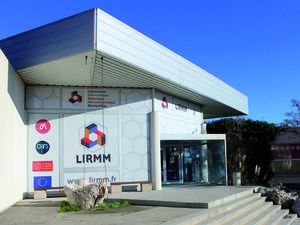
\includegraphics[scale=0.9]{images/lirmmPhoto.jpg}
  \caption{bâtiment 3 du LIRMM, Campus St. Priest}
  \label{fig:lirmmPhoto}
\end{figure}

Les travaux sont menés dans trois départements scientifiques de recherche, [(L’Informatique, La Robotique, et La Microélectronique)] eux-mêmes organisés en \og équipes-projet \fg.

Les recherches menées au LIRMM trouvent généralement une finalisation dans des domaines applicatifs aussi divers que la biologie, la chimie, les télécommunications, la santé, l'environnement... et dans les domaines propres du laboratoire : l'informatique, l'électronique et l'automatique.

Ses activités de recherche [le] positionnent [...] pleinement au coeur des sciences et technologies de l’information, de la communication et des systèmes. [En particulier,] les thématiques du département Informatique s’étendent des frontières des mathématiques à la recherche appliquée : algorithmique des graphes, bioinformatique, cryptographie, réseaux, bases de données et systèmes d'information [...], génie logiciel [...], intelligence artificielle [...], interaction homme-machine [...]. \fg{} \citep{lirmmPres}

%----------------------------------------------------------------------------------------
%   PROBLÈME, MÉTHODOLOGIE, OUTILS ET PLANNING
%----------------------------------------------------------------------------------------
\chapter{Problème, Méthodologie, Outils et Planning}
%----------------------------------------------------------------------------------------
%   PROBLÈME
%----------------------------------------------------------------------------------------
\section{Problème}
Les gens cherchent de \textit{plus en plus} d'acheter des produits frais minimisant les étapes de \textit{processing}, alors que les producteurs cherchent à se libérer des centres d’achat et des intermédiaires de distribution.

Dans l’esprit du site francais \href{https://laruchequiditoui.fr/fr}{LaRucheQuiDitOui}, on souhaite implémenter une interface sous forme d'un \textbf{site web} permettant, au premier, aux producteurs de vendre leurs produits \textbf{directement} aux consommateurs en se regroupant en des endroits précis afin de proposer d'offres diversifiés de leurs produits.

Le site web offrera ainsi \textbf{tout le nécessaire} aux consommateurs pour effectuer des commandes prépayées et précisera en suite les points de collecte de produits les plus proches.\\
D'autre part, le site offrera aussi aux fournisseurs la possibilité d'organiser ces points, de gérer la mise à jour des
stocks et la mise en vente/prise de commandes par les clients, en se basant sur des algorithmes d'optimisation aidant à l'organisation de la logistique, à la préparation/facturation des commandes et à la redistribution des produits entre les différents producteurs voisins.
%----------------------------------------------------------------------------------------
%   MÉTHODOLOGIE
%----------------------------------------------------------------------------------------
\section{Méthodologie}
Dans le but d'assurer la meilleure gestion de nos ressources en offrant le plus de fonctionnalités possibles aux utilisateurs tout en implémentant progressivement leurs requis et faisant sortir des versions fonctionnelles du site après avoir tester les parties implémentées après chaque itération de développement, nous avons opté pour une approche basée sur les \textbf{méthodes agiles} de développement et \textbf{XP}\footnote{\textit{eXtreme Programming}}.

En effet, la méthodologie de développement proposée par les méthodes agiles étant de plus en plus prépondérante en génie logiciel, nous avons décidé d'en profiter pour la modélisation et l'implémentation ultérieure de notre site web pour assurer le plus de flexibilité et d'extensibilité possible lors du dialect développeurs/utilisateurs permettant de répondre efficacement aux besoins des utilisateurs.
%----------------------------------------------------------------------------------------
%   OUTILS
%----------------------------------------------------------------------------------------
\section{Outils}
Pour garantir une bonne modélisation du projet, en cohérence avec l'approche de la méthodologie discutée précédemment, on aura besoin d'expliciter les spécifications fonctionnelles et organisationnelles de notre projet. Ainsi, on aura recours aux outils suivants :
\begin{description}
  \item[\textit{user stories}]{des requis fournis par les utilisateurs décrivant en langage naturel les fonctionnalités qu'il souhaitent avoir dans le site.}
  \item[diagrammes de cas d'usage]{des diagrammes dynamiques, souvent utilisés en \textbf{UML} pour décrire en haut niveau les fonctionnalités d'un système, en se servant de notions telles que \textbf{acteurs}, \textbf{cas d'usage}, \textbf{systèmes} et les \textbf{relations} entre chacune de ces entités.}
  \item[modèle EA]{un modèle \textbf{conceptuel} utilisé pour décrire les entités du projet ainsi que les associations décrivant leurs relations et comportements.}
  \item[schéma de base de données]{schéma en modèle \textbf{relationnel} composé des schémas des relations et des contraintes d'intégrité sur l'ensemble des relations, traduit généralement à partir du \textbf{modèle EA}.}
  \item[\textit{mockup storyboard}]{document de haut niveau offrant un moyen pour schématiser l'utilisation d'un projet, en positionant les différents éléments le composant, sans rentrer dans les détails de leur fonctionnement.}
\end{description}

%----------------------------------------------------------------------------------------
%   PLANNING PRÉVISIONNEL
%----------------------------------------------------------------------------------------
\section{Planning prévisionnel}
  %OTHMANE

%----------------------------------------------------------------------------------------
%   CONCEPTION
%----------------------------------------------------------------------------------------
\chapter{Conception}
%----------------------------------------------------------------------------------------
%   USER STORIES
%----------------------------------------------------------------------------------------
\section{\textit{User Stories}}
Dans cette section nous illustrons les \textit{user stories} que nous avons rédigés pour identifier les fonctionnalités du système conçu :
\subsection{Index Page}
\begin{userStory}[Account Creation]
\textbf{As a {\color{green} client}/{\color{red} vendor} user}, I want to have my own \textbf{personal account},\\
\indent
\textbf{so that} I can have my own \textbf{preferences} and my \textbf{history of purchases/sales}.
\end{userStory}

\begin{userStory}[Account Creation via Other Platforms]
\textbf{As a {\color{green} client}/{\color{red} vendor} user}, I want to be able to \textbf{sign-up} using my \texttt{Facebook}/\texttt{Google} \textbf{account},\\
\indent
\textbf{so that} I don't have to \textbf{fill up forms} and also \textbf{sync my data} between different online platforms.
\end{userStory}

\begin{userStory}[Simultaneous Client/Vendor Account]
\textbf{As a {\color{green} client}/{\color{red} vendor} user}, I want to be able to consult the website as \textbf{both} a \textbf{purchasing client} and a \textbf{vendor} (in case I am both) on the website,\\
\indent
\textbf{so that} I get to \textbf{enjoy the website} in both \textbf{consumption} and \textbf{production} modes without having to sign-off and sign-in every time I want to switch between the modes.
\end{userStory}

\begin{userStory}[Footer Menu]
\textbf{As a {\color{green} client}/{\color{red} vendor} user}, I want to be able to consult a \textbf{menu in the footer of the index page} of the website,\\
\indent
\textbf{so that} I get to learn about the usage of the website through \textbf{FAQs}, understand what I can and cannot do through the \textbf{terms and conditions of usage}, get informed about the \textbf{creators of the website}, \textit{etc...}
\end{userStory}

\subsection{Home Page}
\begin{userStory}[Home Personal Settings]
\textbf{As a {\color{green} client}/{\color{red} vendor} user}, I want a \textbf{personalized user experience} with respect to my \textbf{preferences} and \textbf{history of purchases/sales} in the \textbf{settings},\\
\indent
\textbf{so that} I get to \textbf{visualize information} that are \textbf{relevant to my needs} while simultaneously preserving my \textbf{online privacy}.
\end{userStory}

\subsection{Searching}
\begin{userStory}[Search Results]
\textbf{As a {\color{green} client}/{\color{red} vendor} user}, I want to visualize information about products, vendors, and cells in my search results,\\
\indent
\textbf{so that} I get to have the \textbf{necessary amount of information} about them while surfing for \textbf{products} to \textbf{purchase} or \textbf{vendors/hives} to \textbf{consult}.
\end{userStory}

\begin{userStory}[Search Parameters]
\textbf{As a {\color{green} client}/{\color{red} vendor} user}, I want to \textbf{sort} my \textbf{search results} according to \textbf{parameters} such as stock information, harvest date, expiry date, price, proximity, popularity, vendor, category, list of similar products, etc...,\\
\indent
\textbf{so that} I get to \textbf{personalize} my \textbf{search results} according to my \textbf{needs}.
\end{userStory}

\begin{userStory}[Search Features]
\textbf{As a {\color{green} client}/{\color{red} vendor} user}, I want to use some \textbf{searching features} like \textbf{auto-completion}, \textbf{highlighting}, \textbf{visuals}, etc...,\\
\indent
\textbf{so that} I get to \textbf{search quickly, easily and intuitively} through for information.
\end{userStory}

\subsection{Communication}
\subsubsection{Instant Messaging}
\begin{userStory}[Client $\leftrightarrows$ Vendor and Vendor $\leftrightarrows$ Client/Vendor IM]
\textbf{As a {\color{green} client}/{\color{red} vendor} user}, I want to be able to communicate with a specific client/vendor privately in an instant message environment,\\
\indent
\textbf{so that} I get to \textbf{inquire more about specific information} concerning \textbf{products} or \textbf{hive cells} or other topics.
\end{userStory}

\subsubsection{Email}
\begin{userStory}[Client $\leftrightarrows$ Vendor and Vendor $\leftrightarrows$ Client/Vendor Email]
\textbf{As a {\color{green} client}/{\color{red} vendor} user}, I want to be able to communicate with a specific client/vendor privately via email,\\
\indent
\textbf{so that} my inquiries get to \textbf{reach them as soon as possible} on their \textbf{emails} in case they didn't consult their website account \textbf{regularly}.
\end{userStory}

\subsection{Products \& Logistics}
\subsubsection{Product Review}
\begin{userStory}[Product Reviews]
\textbf{As a {\color{green} client}/{\color{red} vendor} user}, I want to \textbf{consult reviews} (As a {\color{green} client}/{\color{red} vendor} user) about \textbf{products} and write them (As a {\color{green} client} user only),\\
\indent
\textbf{so that} I get to make \textbf{informed purchasing decisions} and \textbf{evaluate the experience} to benefit other future users.
\end{userStory}

\subsubsection{Product Management}
\begin{userStory}[Product Definition and Online Storage]
\textbf{As a {\color{red} vendor} user}, I want to \textbf{define} my \textbf{product selection} according to specific \textbf{descriptive properties} allowing me to divulge as much information about a product as possible,\\
\indent
\textbf{so that} I get to \textbf{maximize transparency} about my products and \textbf{gain customer loyalty} while \textbf{easily and intuitively managing}\footnote{creating, modifying, removing, adding} \textbf{my product selection} through the website.
\end{userStory}

\begin{userStory}[Basket Offers]
\textbf{As a {\color{red} vendor} user}, I would like to \textbf{propose baskets of differents products},\\
\indent
\textbf{so that} I get to offer a \textbf{diversified selection of my products} and \textbf{increase revenue}.
\end{userStory}

\begin{userStory}[Periodical Product Reports]
\textbf{As a {\color{red} vendor} user}, I want to have access to \textbf{statistical reports} about the \textbf{movements of products and stocks},\\
\indent
\textbf{so that} I get to \textbf{analyze the market} and \textbf{define} my \textbf{supply and demand methodology} accordingly.
\end{userStory}

\subsubsection{Logistics}
\begin{userStory}[Depletion of Stock Policy]
\textbf{As a {\color{red} vendor} user}, I want to \textbf{maximize my selling rate} to the point of stocks' \textbf{near-depletion},\\
\indent
\textbf{so that} I get to have the \textbf{least surplus of products in my stock as possible} and make more profit.
\end{userStory}

\begin{userStory}[Hive Product-Sharing Policy]
\textbf{As a {\color{red} vendor} user}, I want to have the possibility of \textbf{exchanging my products with vendors from other cells in the hive}, to offer their products in my cells and have my products offered in theirs,\\
\indent
\textbf{so that} we all benefit from a \textbf{mutual market expansion} and extended revenue surface.
\end{userStory}

\begin{userStory}[Relay and Location-Independent Delivery System]
\textbf{As a {\color{green} client} user}, I want to be capable of having my \textbf{purchases delivered} to a \textbf{desired location nearby a cell collection event} or to a \textbf{fixed relay center of distribution} if possible,\\
\indent
\textbf{so that} I get to collect my purchases \textbf{conveniently} wherever and whenever possible, without having to attend a hive cell collection event myself.
\end{userStory}

\begin{userStory}[Cell Collection Notifications]
\textbf{As a {\color{green} client}/{\color{red} vendor} user}, I want to have the option of \textbf{receiving notifications} about \textbf{hive cell collection events near me}, regardless whether or not I'm supposed to participate in them (not necessarily having purchased anything that I have to collect),\\
\indent
\textbf{so that} I get to know when and where to pick up my purchased products or simply be in touch with \textbf{nearby activity}.
\end{userStory}

\subsection{Order \& Payment}
\subsubsection{Order}
\begin{userStory}[Shopping Cart]
\textbf{As a {\color{green} client} user}, I would like to add the products I wish to purchase to a \textbf{virtual shopping cart},\\
\indent
\textbf{so that} I get to follow my \textbf{shopping progress} and visualize the \textbf{quantity of selected products}, their \textbf{individual prices}, and their \textbf{total price}.
\end{userStory}

\begin{userStory}[Time of Collection Selection]
\textbf{As a {\color{green} client} user}, I would like to choose \textbf{when to collect my purchased products} from the available time slots,\\
\indent
\textbf{so that} I get to collect them \textbf{conveniently} without troubling my personal schedule.
\end{userStory}

\begin{userStory}[Purchase Deadline]
\textbf{As a {\color{red} vendor} user}, I would like to impose specific \textbf{deadlines} on certain product orders,\\
\indent
\textbf{so that} I get to \textbf{customize} my \textbf{supply and demand parameters} while \textbf{processing pending orders} accordingly.
\end{userStory}

\begin{userStory}[Delayed Orders]
\textbf{As a {\color{red} vendor} user}, I would like to offer my customers the chance to make \textbf{delayed orders} for certain \textbf{out-of-stock products},\\
\indent
\textbf{so that} I don't lose my share of the market when certain stocks of products are depleted.
\end{userStory}

\begin{userStory}[Order Validation]
\textbf{As a {\color{red} vendor} user}, I would like to \textbf{manually} or \textbf{automatically validate purchase transactions},\\
\indent
\textbf{so that} I get to \textbf{customize} my \textbf{control} over the \textbf{transactions} according to my \textbf{products stocks}.
\end{userStory}

\subsubsection{Payment}
\begin{userStory}[Payment Methods]
\textbf{As a {\color{green} client} user}, I would like to have \textbf{secure online payment methods} through my \textbf{personal bank}/\texttt{PayPal} \textbf{account},\\
\indent
\textbf{so that} I \textbf{protect my financial credentials} and \textbf{complete my purchases reliably}.
\end{userStory}

\begin{userStory}[Digital Wallet]
\textbf{As a {\color{green} client} user}, I would like to have a \textbf{digital wallet associated to my own personal account} that contains digital currency points I collect from my website activity,\\
\indent
\textbf{so that} I benefit from \textbf{reductions} while purchasing certain products, defined according to the \textbf{number of points} I have \textbf{collected} through my website activity.
\end{userStory}

\begin{userStory}[Vendor Automatic Money Transfer]
\textbf{As a {\color{red} vendor} user}, I would like to have the \textbf{money} gained at the end of a transaction \textbf{transferred directly} into my bank/\texttt{Paypal} account,\\
\indent
\textbf{so that} I get to \textbf{update} my bank \textbf{balance automatically}.
\end{userStory}

\begin{userStory}[Receipt]
\textbf{As a {\color{green} client}/{\color{red} vendor} user}, I would like to receive a \textbf{receipt} at the end of a \textbf{transaction} via \textbf{sms} and \textbf{email}, and have my \textbf{history of purchases/sales updated},\\
\indent
\textbf{so that} I get to keep \textbf{track} of my \textbf{purchases/sales} through \textbf{different media} for larger \textbf{accessibility} and \textbf{data integrity}.
\end{userStory}

\begin{userStory}[Purchase Cancellation \& Reimbursment Policy]
\textbf{As a {\color{green} client} user}, I would like to have the possibility of \textbf{cancelling a purchase} within a \textbf{specific period} of its occurrence,\\
\indent
\textbf{so that} I would get a \textbf{full/partial reimbursement} following the faulty purchase.
\end{userStory}

%----------------------------------------------------------------------------------------
%   DIAGRAMMES USE-CASE
%----------------------------------------------------------------------------------------
\section{Diagrammes \textit{use-case}}
\subsection{Page d'accueil du site}
Le diagramme \textit{use-case} correspondant aux \textit{user-stories} sur la page d'accueil du site est dans la figure \ref{fig:index_page_case_diagram}.
\begin{figure}[!ht]
  \centering
  \begin{tikzpicture}
    \umlactor{User}
    \umlactor[x=12, y=-3]{External Sign-up Platform}
    \umlactor[x=12, y=-1]{Database}
    \begin{umlsystem}[x=4, fill=red!10]{index page}
      \umlusecase{Sign-up}
      \umlusecase[y=-2, width=2.5cm]{Sign-up via external plaftorm}
      \umlusecase[y=-5]{Sign-in}
      \umlusecase[x=4, width=1.5cm]{Create database entry}
      \umlusecase[x=4, y=-4, width=1.5cm]{Verify credentials}
      \umlusecase[y=-7]{Footer menu}
    \end{umlsystem}
    \umlassoc{User}{usecase-1}
    \umlassoc{User}{usecase-2}
    \umlassoc{User}{usecase-3}
    \umlassoc{User}{usecase-6}
    \umlassoc{External Sign-up Platform}{usecase-2}
    \umlassoc{Database}{usecase-4}
    \umlassoc{Database}{usecase-5}
    \umlinclude{usecase-1}{usecase-4}
    \umlinclude{usecase-2}{usecase-4}
    \umlinclude{usecase-3}{usecase-5}
  \end{tikzpicture}
  \caption{Use case diagram of index page functionalities.}
  \label{fig:index_page_case_diagram}
\end{figure}

\subsection{Page d'accueil des utilisateurs}
Le diagramme \textit{use-case} correspondant aux \textit{user-stories} sur la page d'accueil des utilisateurs (client/vendeur) du site est dans la figure \ref{fig:home_page_use_case_diagram}
\begin{figure}[!ht]
  \centering
  \begin{tikzpicture}
    \setcounter{tikzumlUseCaseNum}{0}
    \umlactor{User}
    \umlactor[y=-4]{Vendor}
    \umlactor[x=9, y=-1]{Database}
    \begin{umlsystem}[x=4, fill=green!10]{home page}
      \umlusecase[width=2cm]{Display Products, Hive Events}
      \umlusecase[x=2, y=-3, width=2cm]{Display Stock/Hive Information}
      \umlusecase[y=-6]{Search}
      \umlusecase[y=-8]{Footer menu}
    \end{umlsystem}
    \umlinherit{Vendor}{User}
    \umlextend{usecase-2}{usecase-1}
    \umlassoc{User}{usecase-1}
    \umlassoc{Vendor}{usecase-2}
    \umlassoc{User}{usecase-3}
    \umlassoc{User}{usecase-4}
    \umlassoc{Database}{usecase-1}
    \umlassoc{Database}{usecase-3}
  \end{tikzpicture}
  \caption{Use case diagram of Home Page functionalities.}
  \label{fig:home_page_use_case_diagram}
\end{figure}

\subsection{Recherche}
Le diagramme \textit{use-case} correspondant aux \textit{user-stories} sur la recherche au sein du site est dans la figure \ref{fig:search_use_case_diagram}
\begin{figure}[!ht]
  \centering
  \begin{tikzpicture}
    \setcounter{tikzumlUseCaseNum}{0}
    \umlactor[x=-1]{User}
    \umlactor[x=10]{Database}
    \begin{umlsystem}[x=4, fill=green!10]{home page}
      \umlusecase{Search}
      \umlusecase[x=-2, y=-3, width=2cm]{Choose Search Parameters}
      \umlusecase[x=2, y=-3, width=2cm]{Activate Search Features}
    \end{umlsystem}
    \umlextend[name=ext]{usecase-2}{usecase-1}
    \umlextend[name=ext2]{usecase-3}{usecase-1}
    \umlassoc{User}{usecase-1}
    \umlassoc{User}{usecase-2}
    \umlassoc{User}{usecase-3}
    \umlassoc{Database}{usecase-1}
    \umlassoc{Database}{usecase-2}
    \umlassoc{Database}{usecase-3}
    \umlnote[x=-2, y=-6]{ext-1}{default parameters, else check what parameters to use}
    \umlnote[x=10, y=-6]{ext2-1}{activated by default, else disable in settings}
  \end{tikzpicture}
  \caption{Use case diagram of searching functionality.}
  \label{fig:search_use_case_diagram}
\end{figure}

\subsection{Communication}
Les diagrammes \textit{use-case} correspondant aux \textit{user-stories} sur la communication au sein du site sont respectivement dans les figures \ref{fig:instant_messaging_use_case_diagram} et \ref{fig:email_use_case_diagram}.
\begin{figure}[!ht]
  \centering
  \begin{tikzpicture}
    \setcounter{tikzumlUseCaseNum}{0}
    \umlactor{User}
    \umlactor[x=8]{Vendor}
    \begin{umlsystem}[x=4, fill=green!10]{home page}
      \umlusecase{Chat privately}
    \end{umlsystem}
    \umlassoc{User}{usecase-1}
    \umlassoc{Vendor}{usecase-1}
  \end{tikzpicture}
  \caption{Use case diagram of private instant messaging between client/vendor and vendor.}
  \label{fig:instant_messaging_use_case_diagram}
\end{figure}

\begin{figure}[!ht]
  \centering
  \begin{tikzpicture}
    \setcounter{tikzumlUseCaseNum}{0}
    \umlactor{User}
    \umlactor[x=7]{Vendor}
    \umlactor[x=4, y=3]{Email Service Interface}
    \umlactor[x=14]{Email Database}
    \begin{umlsystem}[x=4, fill=green!10]{home page}
      \umlusecase{Send email}
    \end{umlsystem}
    \begin{umlsystem}[x=10, fill=blue!10]{email system}
      \umlusecase{Receive emails}
      \umlusecase[y=-2]{Check inbox}
    \end{umlsystem}
    \umlassoc{User}{usecase-1}
    \umlassoc{Email Service Interface}{usecase-1}
    \umlassoc{Email Service Interface}{usecase-2}
    \umlassoc{Vendor}{usecase-3}
    \umlassoc{Email Database}{usecase-2}
    \umlassoc{Email Database}{usecase-3}
  \end{tikzpicture}
  \caption{Use case diagram of an email functionality between client/vendor and vendor.}
  \label{fig:email_use_case_diagram}
\end{figure}

\subsection{Produits}
Les diagrammes \textit{use-case} correspondant aux \textit{user-stories} sur les produits sont respectivement dans les figures \ref{fig:product_review_use_case_diagram} et \ref{fig:product_management_use_case_diagram}.
\begin{figure}[!ht]
  \centering
  \begin{tikzpicture}
    \setcounter{tikzumlUseCaseNum}{0}
    \umlactor{User}
    \umlactor[y=-4]{Client}
    \umlactor[x=8, y=-1]{Database}
    \begin{umlsystem}[x=4, fill=green!10]{home page}
      \umlusecase{Search}
      \umlusecase[y=-3, width=2cm]{Search for Products}
      \umlusecase[y=-6]{Review Products}
    \end{umlsystem}
    \umlinherit{Client}{User}
    \umlextend{usecase-2}{usecase-1}
    \umlextend[name=ext]{usecase-3}{usecase-2}
    \umlassoc{User}{usecase-1}
    \umlassoc{Client}{usecase-3}
    \umlassoc{Database}{usecase-1}
    \umlassoc{Database}{usecase-3}
    \umlnote[x=9, y=-6]{ext-1}{Only if the user is a client having already purchased the product}
  \end{tikzpicture}
  \caption{Use case diagram of product reviewing functionality.}
  \label{fig:product_review_use_case_diagram}
\end{figure}

\begin{figure}[!ht]
  \centering
  \begin{tikzpicture}
    \setcounter{tikzumlUseCaseNum}{0}
    \umlactor{Vendor}
    \umlactor[x=8, y=-1]{Database}
    \begin{umlsystem}[x=4, fill=green!10]{home page}
      \umlusecase[width=3cm]{Add/Delete/Modify Products}
      \umlusecase[y=-3, width=3cm]{Add/Delete/Modify Baskets}
      \umlusecase[y=-6]{Check Stocks}
      \umlusecase[y=-9]{Check Reports}
    \end{umlsystem}
    \umlextend[name=ext]{usecase-2}{usecase-1}
    \umlextend{usecase-4}{usecase-3}
    \umlassoc{User}{usecase-1}
    \umlassoc{User}{usecase-2}
    \umlassoc{User}{usecase-3}
    \umlassoc{User}{usecase-4}
    \umlassoc{Database}{usecase-1}
    \umlassoc{Database}{usecase-2}
    \umlassoc{Database}{usecase-3}
    \umlassoc{Database}{usecase-4}
    \umlnote[x=-2, y=-4]{ext-1}{Products have to exist in the database prior to the introduction of baskets}
  \end{tikzpicture}
  \caption{Use case diagram of product management functionality.}
  \label{fig:product_management_use_case_diagram}
\end{figure}

\subsection{Commandes \& Paiement}
Les diagrammes \textit{use-case} correspondant aux \textit{user-stories} sur les commandes et paiements sont respectivement dans les figures \ref{fig:order_payment_client_use_case_diagram} et \ref{fig:order_payment_vendor_use_case_diagram}.
\begin{figure}[!ht]
  \centering
  \begin{tikzpicture}
    \setcounter{tikzumlUseCaseNum}{0}
    \umlactor{Client}
    \umlactor[y=-4]{Database}
    \umlactor[x=14, y=-6.2]{Vendor User Database}
    \umlactor[x=14, y=-11]{Money Payment Platform}
    \umlactor[x=8, y=-14]{Bill Reception Platform}
    \umlactor[x=4.5, y=-14]{Bank/PayPal}
    \begin{umlsystem}[x=4, fill=green!10]{client home page}
      \umlusecase[width=2cm] {Add Items to Shopping Cart} %1
      \umlusecase[x=5, width=2cm]{Delete Items from Shopping Cart} %2
      \umlusecase[x=3.5, y=-3, width=2cm]{Choose Time of Collection} %3
      \umlusecase[x=5, y=-6, width=3cm]{Choose Payment Method} %4
      \umlusecase[x=5, y=-9, width=3cm]{Get Reductions from Wallet Points} %5
      \umlusecase[y=-12]{Check Wallet} %6
      \umlusecase[y=-9, width=3cm]{Checkout from Payment} %7
      \umlusecase[y=-6, width=3cm]{Update Purchases' History} %8
      \umlusecase[x=5, y=-12, width=3cm]{Receive Bill} %9
    \end{umlsystem}
    \begin{umlsystem}[x=14.2, fill=red!10]{vendor home page}
      \umlusecase[width=1.5cm]{Send a Bill} %10
    \end{umlsystem}
    \umlextend{usecase-2}{usecase-1}
    \umlextend{usecase-5}{usecase-4}
    \umlinclude{usecase-1}{usecase-3}
    \umlinclude{usecase-3}{usecase-4}
    \umlinclude{usecase-7}{usecase-8}
    \umlinclude[pos stereo=0.2]{usecase-9}{usecase-8}
    \umlassoc{Client}{usecase-1}
    \umlassoc{Client}{usecase-6}
    \umlassoc{Money Payment Platform}{usecase-4}
    \umlHVassoc{Money Payment Platform}{usecase-7}
    \umlassoc{Vendor User Database}{usecase-7}
    \umlassoc{Vendor User Database}{usecase-9}
    \umlassoc[name=send]{Vendor User Database}{usecase-10}
    \umlassoc{Bill Reception Platform}{usecase-9}
    \umlassoc{Bank/PayPal}{usecase-9}
    \umlassoc{Database}{usecase-8}
    \umlnote[x=12, y=-3]{send-1}{only if transaction validated by vendor}
  \end{tikzpicture}
  \caption{Use case diagram of Order and Payment functionalities viewed from the client user side.}
  \label{fig:order_payment_client_use_case_diagram}
\end{figure}

\begin{figure}[!ht]
  \centering
  \begin{tikzpicture}
    \setcounter{tikzumlUseCaseNum}{0}
    \umlactor{Vendor}
    \umlactor[x=13, y=-2]{Database}
    \umlactor[y=-13]{Client User Database}
    \umlactor[x=13, y=-11]{Bill Reception Platform}
    \umlactor[x=4.5, y=-13]{Bank/PayPal}
    \begin{umlsystem}[x=4, fill=red!10]{vendor home page}
      \umlusecase[width=2cm]{Check Stocks}
      \umlusecase[x=5, width=2cm]{Allow Delayed Orders}
      \umlusecase[x=3.5, y=-3, width=3cm]{Set Purchase Deadline}
      \umlusecase[x=4, y=-6, width=3cm]{Check Pending Orders}
      \umlusecase[y=-8, width=2cm]{Process Pending Orders}
      \umlusecase[x=5, y=-8, width=2cm]{Send Bill}
      \umlusecase[x=4.5, y=-11, width=2cm]{Update Sales' History}
    \end{umlsystem}
    \umlextend{usecase-2}{usecase-1}
    \umlextend[name=deadline]{usecase-3}{usecase-4}
    \umlextend[name=checkPending1]{usecase-4}{usecase-5}
    \umlinclude{usecase-5}{usecase-6}
    \umlinclude{usecase-6}{usecase-7}
    \umlassoc{Vendor}{usecase-1}
    \umlassoc[name=checkPending2]{Vendor}{usecase-4}
    \umlassoc[name=process]{Vendor}{usecase-5}
    \umlassoc{Database}{usecase-2}
    \umlassoc{Database}{usecase-3}
    \umlassoc{Database}{usecase-4}
    \umlassoc{Database}{usecase-7}
    \umlassoc{Bill Reception Platform}{usecase-6}
    \umlassoc{Bank/PayPal}{usecase-6}
    \umlassoc{Client User Database}{usecase-6}
    \umlnote[x=-1, y=-5]{checkPending1-1}{only if validating transactions is set to manual}
    \umlnote[x=-1, y=-5]{checkPending2-1}{only if validating transactions is set to manual}
    \umlnote[x=-1, y=-8]{process-1}{only if validating transactions is set to automatic}
    \umlnote[x=-1, y=-11]{deadline-1}{according to the number of pending orders}
  \end{tikzpicture}
  \caption{Use case diagram of Order and Payment functionalities viewed from the vendor user side.}
  \label{fig:order_payment_vendor_use_case_diagram}
\end{figure}
%----------------------------------------------------------------------------------------
%   SD PROPOSÉE (CELLULE ET RUCHE)
%----------------------------------------------------------------------------------------
\section{Structure de données proposée (\texttt{Cellule} et \texttt{Ruche})}
Afin de pouvoir optimiser la logistique et la redistribution des produits entre les fournisseurs à proximité l'un de l'autre, il va falloir proposer une \textbf{structure de données} permettant d'abstraire la notion de \textbf{ruche} et étudier ses propriétés et opérations afin d'analyser ses avantages et inconvénients par rapport à nos besoins.

\subsection{Définitions et notations}
\begin{description}
  \item[$V$]{ensemble des fournisseurs.}
  \item[$Cl$]{ensemble des clients.}
  \item[$C$]{\textbf{opérateur} appliqué à $v \in V$ désignant une \textbf{cellule}, ç-à-d un \textbf{cercle} dont le centre est le point représentant les coordonnées du fournisseur $v$ et dont le rayon est la distance maximale en \textbf{km} qu'il souhaite parcourir pour rendre ces produits à un point de collecte.}
\end{description}

\begin{definition}[Ruche]
Soit $v_1, v_2, \dots, v_n \in V^n$. Une \textbf{ruche} $R$ est composée d'un ensemble de fournisseurs dont les cellules s'intersectent et d'un point de collecte obtenu à partir d'une opération sur le polygone dont les sommets correspondent aux cellules de chaque vendeur.\\
Autrement dit, $R = \{p, v_1, v_2, \dots, v_n \in V\; |\; C(v_1) \cap C(v_2) \cap \dots \cap C(v_n) \neq \varnothing\}$
\end{definition}

\begin{property}[Fournisseurs Voisins]
Soit $R$ une ruche. Deux fournisseurs $v_1$ et $v_2$ sont dits \textbf{voisins} $\iff v_1 \in R\; \text{et}\; v_2 \in R$. On note $\texttt{Voisins}(v)$ l'\textbf{ensemble des voisins} d'un fournisseur $v \in V$.
\end{property}

\begin{constraint}[Chevauchement des ruches]
Un fournisseur peut appartenir à plusieurs ruches $R_1, R_2, \dots, R_k$ simultanément.
\end{constraint}

\begin{constraint}[Voisinage Imposé]
Soient $v_1$ et $v_2$ deux fournisseurs tels que $v_2 \notin \texttt{Voisins}(v_1)$. S'il existe des fournisseurs $v_3$ et $v_4$ tels que $v_3, v_4 \in \texttt{Voisins}(v_1) \cap \texttt{Voisins}(v_2)$, alors il existe une ruche plus optimale contenant $v_1, v_2, v_3\; \text{et}\; v_4$ que les ruches séparées les contenant.
\end{constraint}
%----------------------------------------------------------------------------------------
%   MODÈLE EA
%----------------------------------------------------------------------------------------
\section{Modèle EA}

%----------------------------------------------------------------------------------------
%   SCHÉMA DE BD
%----------------------------------------------------------------------------------------
\section{Schéma de base de données}
Le modèle relationnel obtenu par traduction du modèle EA des données est le suivant :
\begin{enumerate}
  \item{\texttt{CLIENT}(\underline{email}, nom, prenom, adresse, codePostale, Ville, Pays).}
  \item{\texttt{WALLET}(\underline{ID\_wallet}, \textit{emailClient}).}
  \item{\texttt{VENDOR}(\underline{emailV}, siret, nomProfessionel).}
  \item{\texttt{STOCK}(\underline{ID\_stock}, \underline{emailV}).}
  \item{\texttt{BASKET}(\underline{ID\_basket}).}
  \item{\texttt{TYPE\_PRODUCT}(ID\_typeP).}
  \item{\texttt{PRODUCT}(\underline{ID\_product}, name, \textit{ID\_stock}, \textit{ID\_typeP}, \textit{ID\_basket}).}
  \item{\texttt{SUBORDER}(\underline{ID\_suborder}, isValidated, \textit{ID\_order}, \textit{emailV}).}
  \item{\texttt{CONTAINS}(\underline{\textit{ID\_suborder}}, \underline{\textit{ID\_product}}, quantity).}
  \item{\texttt{PAYMENTMETHOD}(\underline{ID\_paymentMethod}).}
  \item{\texttt{STATUS}(\underline{ID\_status}).}
  \item{\texttt{ORDER}(\underline{ID\_order}, dateOrder, \textit{emailClient}, \textit{ID\_wallet}, walletPoints, \textit{ID\_paymentMethod}, \textit{ID\_status}).}
\end{enumerate}

%----------------------------------------------------------------------------------------
%   STORYBOARD
%----------------------------------------------------------------------------------------
\section{Storyboard}

%----------------------------------------------------------------------------------------
%   CONCLUSION
%----------------------------------------------------------------------------------------
\chapter{Conclusion}
%----------------------------------------------------------------------------------------
%   IMPLÉMENTATION PRÉVUE
%----------------------------------------------------------------------------------------
\section{Implémentation prévue}
Pour la mise en oeuvre du site web, on prévoit utiliser, à part \textbf{HTML} et \textbf{CSS}, les outils suivants :
\begin{enumerate}
  \item{\textbf{JavaScript} et des \textbf{\textit{frameworks} pertinents} tels que \textbf{JQuery} et \textbf{Angular}, utilisés pour le développement \textit{front-end} du site web.}
  \item{le \textbf{\textit{framework} Bootstrap} pour faire des pages responsives adaptables aux dispositifs tels que smartphones, tablets, laptops et grand écrans.}
  \item{\textbf{MySQL} pour gérer la base de données du site : on a opté pour une BD relationnel vu le grand nombre d'associations reliant les différentes entités du site.}
  \item{\textbf{PHP} : suite au choix de \textbf{MySQL}, \textbf{PHP} (ainsi que les \textbf{\textit{frameworks}} basés dessus et \textbf{ORM}) est l'un des langages côté serveur les plus adaptés et les plus utilisés pour la manipulation d'un SGBD relationnel.}
\end{enumerate}

\begin{remark}
L'utilisation des \textbf{API} est aussi contemplée, notamment pour l'implémentation d'une carte (\textbf{Leaflet}), d'un chat securisé (\textbf{Telegram}), des méthodes de paiement, \textit{etc...}
\end{remark}
%----------------------------------------------------------------------------------------
%   PERSPECTIVES
%----------------------------------------------------------------------------------------
\section{Perspectives}
En plus des fonctionnalités que nous avons jugées être essentielles au projet et que nous prévoyons donc d'implémenter, nous avons pensé à des fonctionnalités supplémentaires que nous pourrions ajouter à notre projet une fois celles de base établies.

En effet, plusieurs extensions sont possibles afin de proposer aux utilisateurs du site un choix plus diversifié.
Parmi celles-ci nous avons pensé au fait de proposer aux clients réalisant des achats sur le site d'avoir la possibilité de régler, en plus qu'avec un paiement bancaire, de pouvoir recourir à des services de paiements en ligne telles que Paypal,
voire même d'offrir la possibilité de payer en Crypto-monnaie dans une version plus développée du projet.

Outre cela, nous pourrions également proposer plusieurs versions de notre site, où chaque version concerne un pays particulier et donc dans une langue précise.\\
Tout cela, dans le but de pouvoir déployer le site ainsi que son concept à l'international.
%----------------------------------------------------------------------------------------
%   BIBLIOGRAPHIE
%----------------------------------------------------------------------------------------
\bibliographystyle{agsm}
\bibliography{mybib}

\end{document}
